\section{Durchführung}
\label{sec:Durchführung}
%\subsection{Aufbau}
%Die Schwebungen werden mit einem Schwingkreis, wie in Abbildung \ref{fig:1}, untersucht.








\subsection{Justierungen}
\label{sec:d0}
Die Schwebungen werden mit einem Schwingkreis, wie in Abbildung \ref{fig:schwingkreis} aus der Theorie, untersucht.
Bevor die Messreihen beginnen, müssen gewisse Justierungen getroffen werden.
Um, wie in der Theorie beschrieben, einen möglichst guten Energieaustausch zu gewährleisten, sollten die beiden Schwingkreise die selbe Resonanzfrequenz besitzen.
Dazu wird zuerst die Schaltung aus Abbildung \ref{fig:2} nachgebaut.

\begin{figure}[H]
  \centering
  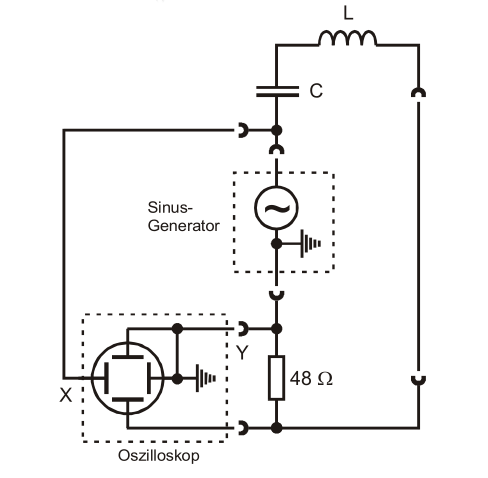
\includegraphics[height=6cm]{just1.png}
  \caption{linke Masche. \cite{sample}}
  \label{fig:2}
\end{figure}

Sie besteht aus einem Sinusgenerator und jeweils dazu einen in Reihe geschalteten Kondensator und einer Spule.
Ein Oszilloskop misst nach der Spule an einem Ohmschen Widerstand die Spannung über den Y-Eingang.
Dessen X-Eingang wird zwischen Generator und Kondensator zugesteckt.
Sie repräsentiert die linke Masche des gesamten Schwingkreises, wobei der Kondensator $C_k$ überbrückt wird.\\
Eine Resonanz liegt vor wenn die Phase zwischen Generatorspannung und Schwingkreisstrom 0 beziehungsweise $\pi$ ist.
Dies wird über die Lissajous-Figur über das Oszilloskop bestimmt.
Nun wird die Frequenz der Sinusspannung solange variiert, bis die Resonanz des Schwingkreises beobachtet wird.
Die Frequenz wird vermerkt.
Als nächstes wird die rechte Seite des gesamten Schwingkreises aufgebaut, die in Abbildung \ref{fig:3} dargestellt wird.

\begin{figure}[H]
  \centering
  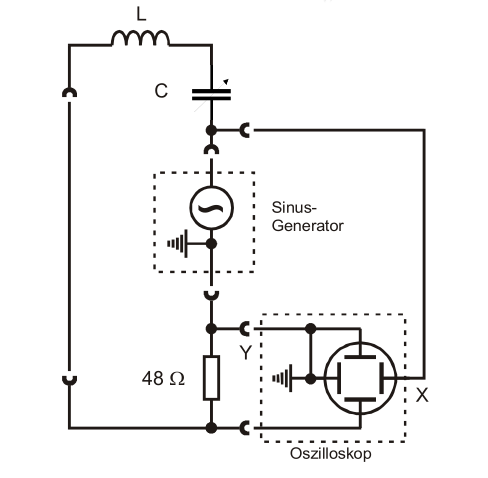
\includegraphics[height=6cm]{just2.png}
  \caption{rechte Masche.}
  \label{fig:3}
\end{figure}

Es befindet sich jedoch an Stelle eines festen ein regelbarer Kondensator in der Schaltung.\\
Dieser Schwingkreis wird nun mit der Resonanzfrequenz des linken betrieben.
Hierbei wird jedoch die Kapazität des Kondensators variiert, bis erneut eine Resonanz erzeugt wird.
Die beiden Maschen haben nun die selbe Resonanzfrequenz und sind somit aufeinander abgestimmt.
Die Messreihe kann nun beginnen.\\
\subsection{Bestimmung der Schwebungsfrequenzen}
\label{sec:d1}
Nun wird der gesamte Aufbau betrachtet.
Die beiden Maschen werden über den gemeinsamen, nun zugeschalteten Koppelkondensator $C_k$ miteinander verbunden.
Der Generator liegt nun wieder an der linken Masche an.
Die Abbildung \ref{fig:4} realisiert dies.

\begin{figure}[H]
  \centering
  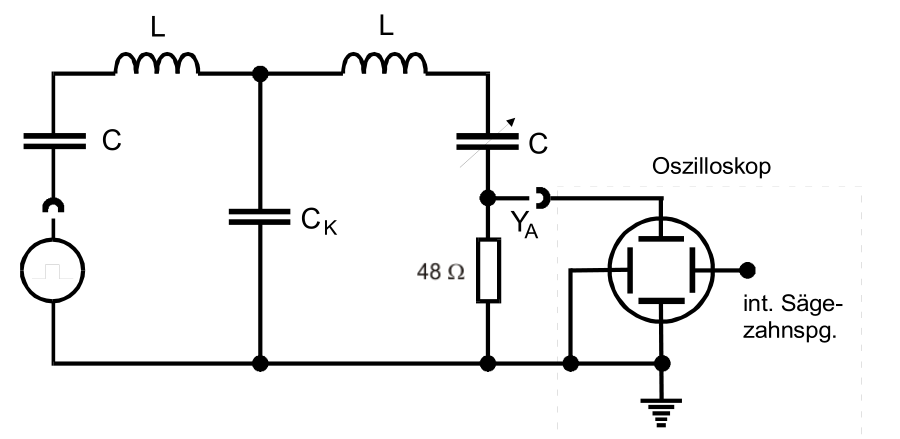
\includegraphics[height=6cm]{a.png}
  \caption{1. Messreihe. \cite{sample}}
  \label{fig:4}
\end{figure}

Der linke Schwingkreis wird extern mittels Rechtecksignal zum Schwingen angeregt.
Auf dem Oszilloskop können die Schwebungen beobachtet werden.
Die Maxima innerhalb einer Schwebung werden notiert.
An ihnen kann das Verhältnis zwischen Schwingungs- und Schwebungsfrequenz abgelesen werden.
Die Messreihe kommt zustande, indem $C_k$ in einem bestimmten Bereich variiert wird.\\
\subsection{Bestimmung der Fundamentalfrequenzen}
\label{sec:d2}
Als Nächstes werden die Frequenzen der Fundamentalschwingung in Abhängigkeit der Kapazität des Koppelkondensators $C_k$ gemessen.
Hierzu wird die Schaltung aus Abbildung \ref{fig:5} nachgebaut.

\begin{figure}[H]
  \centering
  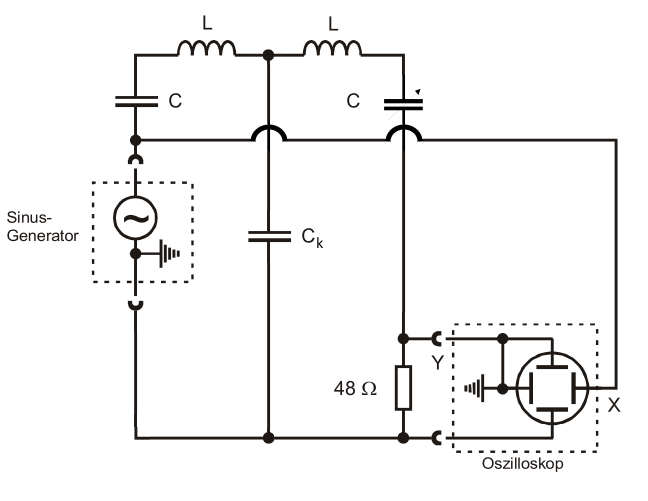
\includegraphics[height=6cm]{b.png}
  \caption{2. und 3. Messreihe.}
  \label{fig:5}
\end{figure}

Der Generator führt dem Stromkreis wieder eine Sinusspannung zu, die von dem X-Eingang des Oszilloskops abgegriffen wird.
Jetzt wird über die Lissajous-Figur die Resonanzfrequenz ermittelt.
Dies wird wider für verschiedene $C_k$ wiederholt.\\
\subsection{Bestimmung eines Frequenzspektrums}
\label{sec:d3}
Zuletzt soll der Verlauf der beiden Ströme $I_2$ und $I_k$ untersucht werden.
Dazu wird der selbe Aufbau wie zuvor, dargestellt in Abbildung \ref{fig:5}, verwendet.
Nun wird jedoch ein Frequenzspektrum durchlaufen.
Auf dem Oszilloskop erscheinen dementsprechend die beiden Resonanzpeaks in Abhängigkeit von der Zeit.
Die Zeiten von der Startfrequenz bis zum Erreichen der Peaks wird notiert.
Dies sollte bestenfalls für mehrere $C_k$ Werte wiederholt werden, wird aus Zeitgründen jedoch unterlassen.
%Ebenfalls unterlassen wird die Messung der Strommaxima.
